% !TEX encoding = UTF-8 Unicode

\documentclass[a4paper]{article}

\usepackage{color}
\usepackage{url}
\usepackage[utf8]{inputenc} % make weird characters work
\usepackage{graphicx}
\usepackage[english,serbian]{babel}
\usepackage[unicode]{hyperref}
\usepackage{amsthm}
\usepackage{amssymb}
\hypersetup{colorlinks,citecolor=green,filecolor=green,linkcolor=blue,urlcolor=blue}
\usepackage[title]{appendix}
\usepackage{float}
\usepackage[graphicx]{realboxes}
\usepackage[font=small,labelfont=bf]{caption}
\usepackage{chngcntr}
\counterwithin{figure}{section}
\usepackage{listings}
\definecolor{codegreen}{rgb}{0,0.6,0}
\definecolor{codegray}{rgb}{0.5,0.5,0.5}
\definecolor{codeblue}{rgb}{0.0,0,0.82}
\lstdefinestyle{mystyle}{
    numbers=left,
    numberstyle=\scriptsize,
    numbersep=8pt,
    commentstyle=\color{codegray},
    keywordstyle=\color{codegreen},
    numberstyle=\tiny\color{codeblue},
    stringstyle=\color{codegreen},
    basicstyle=\ttfamily\footnotesize,
    breakatwhitespace=false,
    breaklines=true,
    captionpos=b,
    keepspaces=true,
    showspaces=false,
    showstringspaces=false,
    showtabs=false,
    tabsize=4,
    xleftmargin=3em,
    framexleftmargin=1.5em
}
\lstset{style=mystyle}


\begin{document}

\title{Analiza ``Million Songs'' skupa podataka\\ \small{Seminarski rad u okviru kursa\\Istra\v{z}ivanje podataka\\ Matematički fakultet}}

\author{\href{mailto:mi14031@matf.bg.ac.rs}{Milana Kova\v{c}evi\'c}\\\href{mailto:mi14042@matf.bg.ac.rs}{Ivan Ristovi\'c}}
\date{jun 2018.}

\maketitle

\abstract{
U ovom radu \c'{}emo istra\v{z}ivati skup podataka \emph{Million Songs Dataset}. Milana molim te pomozi
Lorem ipsum dolor sit amet, consectetur adipisicing elit, sed do eiusmod tempor incididunt ut labore et dolore magna aliqua. Ut enim ad minim veniam, quis nostrud exercitation ullamco laboris nisi ut aliquip ex ea commodo consequat. Duis aute irure dolor in reprehenderit in voluptate velit esse cillum dolore eu fugiat nulla pariatur. Excepteur sint occaecat cupidatat non proident, sunt in culpa qui officia deserunt mollit anim id est laborum.
}


\tableofcontents

\newpage

\section{Opis skupa podataka}
\label{sec:Opis skupa podataka}

\emph{The Million Song Dataset} \cite{Dataset} je skup od milion slogova koji sadr\v{z}e informacije o popularnim pesmama. S obzirom da ovaj skup preveliki za udoban rad, ograni\v{c}i\'c{}emo se na podskup od deset hiljada slogova izdvojen od strane autora originalnog skupa.

Svaki slog pomenutog skupa podataka sadr\v{z}i informacije o jednoj pesmi: detalje o izvodja\v{c}u, segmentima, tempu kao i ID pesme na raznim online servisima (\emph{Echo Nest} \cite{EchoNest}, \emph{7digital} \cite{7digital},  \emph{MusicBrainz} \cite{MusicBrainz} i \emph{PlayMe} \cite{PlayMe}). Detaljne informacije o atributima se mogu videti na slici \ref{fig:Atributi}.

Skup u svojoj originalnoj formi je organizovan u \emph{HDF5} format \cite{HDF5}. Mi \'c{}emo izdvojiti informacije iz datog modela i podatke organizovati u CSV format, zarad lak\v{s}eg ubacivanja u alate koje \'c{}emo opisati kasnije. Ova transformacija je izvr\v{s}ena kori\v{s}\'c{}enjem Git repozitoriujma MSongsDB koji se mo\v{z}e na\'c{}i na adresi \ref{MSongsDB} podataka i njihova konverzija u CSV format je izvr\v{s}ena kori\v{s}\'c{}enjem Python programa koji se mogu na\'c{}i u dodatku \ref{sec:DodatakIzvlacenje}.


\begin{figure}
    \footnotesize
    \begin{tabular}{|c|c|c|}
        \hline
        Atribut & Tip podatka & Kratki opis \\
        \hline
        analysis sample rate & float & u\v{c}estalost uzorkovanja \\
        artist 7digitalid & int & \emph{7digital} ID izvodja\v{c}a ili -1 \\
        artist familiarity & float & algoritamska aproksimacija \\
        artist hotttnesss & float & algoritamska aproksimacija \\
        artist id & string & \emph{Echo Nest} ID izvodja\v{c}a \\
        artist latitude & float & geografska \v{s}irina \\
        artist location & string & lokacija autora \\
        artist longitude & float & geografska du\v{z}ina \\
        artist mbid & string & MusicBrainz ID izvodja\v{c}a \\
        artist mbtags & array string & niz MusicBrainz tagova \\
        artist mbtags count & array int & broj MusicBrainz tagova \\
        artist name & string & ime autora \\
        artist playmeid & int & \emph{PlayMe} ID izvodja\v{c}a ili -1 \\
        artist terms & array string & niz \emph{Echo Nest} tagova \\
        artist terms freq & array float & frekvencije \emph{Echo Nest} tagova \\
        artist terms weight & array float & te\v{z}ina \emph{Echo Nest} tagova \\
        audio md5 & string & MD5 he\v{s} kod audio zapisa \\
        bars confidence & array float & pouzdanost takta \\
        bars start & array float & niz po\v{c}etaka taktova \\
        beats confidence & array float &pouzdanost ritma \\
        beats start & array float & niz po\v{c}etaka ritmova \\
        danceability & float & algoritamska aproksimacija \\
        duration & float & trajanje audio zapisa (u sekundama) \\
        end of fade in & float & vreme u odnosu na pocetak u kom prestaje\\
        & & fade-in efekat (u sekundama) \\
        energy & float & algoritamska aproksimacija energije \\
        & & pesme od strane slu\v{s}aoca \\
        key & int & tonalitet u kojem je audio zapis \\
        key confidence & float & pouzdanost tonaliteta \\
        loudness & float & prose\v{c}na ja\v{c}ina (u dB) \\
        mode & int & mod - dur ili mol \\
        mode confidence & float & pouzdanost moda \\
        release & string & ime albuma \\
        release 7digitalid & int & \emph{7digital} ID albuma ili -1 \\
        sections confidence & array float & niz pouzdanosti stihova \\
        sections start & array float & po\v{c}eci stihova \\
        segments confidence & array float & niz pouzdanosti segmenata \\
        segments loudness max & array float & nig maksimalnih ja\v{c}ina unutar \\
        & & segmenata (u dB) \\
        segments loudness max time & array float & niz vremena dostizanja maksimalne ja\v{c}ine \\
        & & unutar segmenata \\
        segments loudness max start & array float & niz ja\v{c}ina na po\v{c}ecima segmenata \\
        segments pitches & 2D array float & niz ja\v{c}ina po segmentima, jedna \\
        & & vrednost za svaku notu \\
        segments start & array float & po\v{c}eci segmenata \\
        segments timbre & 2D array float & informacije o teksturi $(MFCC+PCA)$ \\
        similar artists & array string & niz \emph{Echo Nest} sli\v{c}nih izvodja\v{c}a \\
        song hotttnesss & float & algoritamska aproksimacija \\
        song id & string & \emph{Echo Nest} ID pesme \\
        start of fade out & float & vreme u odnosu na pocetak u kom po\v{c}inje \\
        & & fade-out efekat (u sekundama) \\
        tatums confidence & array float & pouzdanost najmanjih elemenata ritma \\
        tatums start & array float & niz najmanjih elemenata ritma \\
        tempo & float & procenjen tempo (u BPM) \\
        time signature & int & procenjen broj ritmova u taktu, npr. 4 \\
        time signature confidence & float & pouzdanost procene broja ritmova u taktu \\
        title & string & naziv pesme \\
        track id & string & \emph{Echo Nest} ID pesme \\
        track 7digitalid & int & ID \emph{7digital} ID pesme ili -1 \\
        year & int & godina izdavanja uzeta sa \emph{MusicBrainz} ili 0 \\
        \hline
    \end{tabular}
    \label{fig:Atributi}
    \caption{Atributi prisutni u \emph{The Million Song Dataset} skupu podataka}
\end{figure}

Primer sloga je prikazan na \ref{primer:Song}. Ovaj prikaz dobijen je pokretanjem displaySong.py skripte koja se nalazi u okviru Git repozitoriujma \ref{MSongsDB}.


\begin{figure}[ht]
%[fontsize=\scriptsize] TODO
\begin{verbatim}
analysis_sample_rate: 22050
artist_7digitalid: 61424
artist_familiarity: 0.5467275539627645
artist_hotttnesss: 0.3861804160792181
artist_id: ARE26EG1187B990AEF
artist_latitude: 51.77045
artist_location: Essex, England
artist_longitude: 0.64255
artist_mbid: de212b3a-2f54-4def-a13d-5a877bfaeaf7
artist_mbtags: shape = (6,)
artist_mbtags_count: shape = (6,)
artist_name: Sunscreem
artist_playmeid: 19156
artist_terms: shape = (44,)
artist_terms_freq: shape = (44,)
artist_terms_weight: shape = (44,)
audio_md5: c2f7f92e66d18e86af3752478d3be966
bars_confidence: shape = (123,)
bars_start: shape = (123,)
beats_confidence: shape = (497,)
beats_start: shape = (497,)
danceability: 0.0
duration: 232.4371
end_of_fade_in: 0.0
energy: 0.0
key: 11
key_confidence: 0.625
loudness: -8.955
mode: 0
mode_confidence: 0.558
release: Looking At You: The Club Anthems
release_7digitalid: 196929
sections_confidence: shape = (6,)
sections_start: shape = (6,)
segments_confidence: shape = (1045,)
segments_loudness_max: shape = (1045,)
segments_loudness_max_time: shape = (1045,)
segments_loudness_start: shape = (1045,)
segments_pitches: shape = (1045, 12)
segments_start: shape = (1045,)
segments_timbre: shape = (1045, 12)
similar_artists: shape = (100,)
song_hotttnesss: nan
song_id: SOICLQB12A8C13637C
start_of_fade_out: 232.437
tatums_confidence: shape = (993,)
tatums_start: shape = (993,)
tempo: 130.201
time_signature: 4
time_signature_confidence: 0.0
title: Exodus
track_7digitalid: 2140010
track_id: TRBBBLA128F424E963
year: 1995

\end{verbatim}
\label{primer:Song}
\caption{Primer sloga iz skupa podataka.}
\end{figure}

\section{Kori\v{s}\'c{}eni alati}
\label{sec:Alati}

Za obradu podataka, kori\'s{}\'c{}eni su alati \emph{Knime Analytics Platform} \cite{KNIME} i \emph{IBM SPSS Modeler} \cite{SPSS}. \emph{IBM SPSS Modeler} je prete\v{z}no kori\v{s}\c'{}en prete\v{z}no za vizuelizaciju, dok je \emph{KNIME AP} kori\'s{}\c'{}en za manipulisanje podacima, vizuelizaciju i primenu algoritama.

\section{Preprocesiranje i analiza podataka}
\label{sec:Preprocesiranje}

Za upotrebu razli\v{c}itih algoritama potrebne su druga\v{c}ije transformacije.

\subsection{Apriori algoritam}
\label{subsec:Apriori}

\begin{itemize}
    \item \emph{Zavisnost \v{z}anra od lokacije}
    \item \emph{Zavisnost \v{z}anra od decenije}
    \item \emph{Zavisnost \v{z}anra od lokacije}
\end{itemize}


Lorem ipsum dolor sit amet, consectetur adipisicing elit, sed do eiusmod tempor incididunt ut labore et dolore magna aliqua. Ut enim ad minim veniam, quis nostrud exercitation ullamco laboris nisi ut aliquip ex ea commodo consequat. Duis aute irure dolor in reprehenderit in voluptate velit esse cillum dolore eu fugiat nulla pariatur. Excepteur sint occaecat cupidatat non proident, sunt in culpa qui officia deserunt mollit anim id est laborum.

Lorem ipsum dolor sit amet, consectetur adipisicing elit, sed do eiusmod tempor incididunt ut labore et dolore magna aliqua. Ut enim ad minim veniam, quis nostrud exercitation ullamco laboris nisi ut aliquip ex ea commodo consequat. Duis aute irure dolor in reprehenderit in voluptate velit esse cillum dolore eu fugiat nulla pariatur. Excepteur sint occaecat cupidatat non proident, sunt in culpa qui officia deserunt mollit anim id est laborum.

Lorem ipsum dolor sit amet, consectetur adipisicing elit, sed do eiusmod tempor incididunt ut labore et dolore magna aliqua. Ut enim ad minim veniam, quis nostrud exercitation ullamco laboris nisi ut aliquip ex ea commodo consequat. Duis aute irure dolor in reprehenderit in voluptate velit esse cillum dolore eu fugiat nulla pariatur. Excepteur sint occaecat cupidatat non proident, sunt in culpa qui officia deserunt mollit anim id est laborum.

Lorem ipsum dolor sit amet, consectetur adipisicing elit, sed do eiusmod tempor incididunt ut labore et dolore magna aliqua. Ut enim ad minim veniam, quis nostrud exercitation ullamco laboris nisi ut aliquip ex ea commodo consequat. Duis aute irure dolor in reprehenderit in voluptate velit esse cillum dolore eu fugiat nulla pariatur. Excepteur sint occaecat cupidatat non proident, sunt in culpa qui officia deserunt mollit anim id est laborum.

Lorem ipsum dolor sit amet, consectetur adipisicing elit, sed do eiusmod tempor incididunt ut labore et dolore magna aliqua. Ut enim ad minim veniam, quis nostrud exercitation ullamco laboris nisi ut aliquip ex ea commodo consequat. Duis aute irure dolor in reprehenderit in voluptate velit esse cillum dolore eu fugiat nulla pariatur. Excepteur sint occaecat cupidatat non proident, sunt in culpa qui officia deserunt mollit anim id est laborum.

Lorem ipsum dolor sit amet, consectetur adipisicing elit, sed do eiusmod tempor incididunt ut labore et dolore magna aliqua. Ut enim ad minim veniam, quis nostrud exercitation ullamco laboris nisi ut aliquip ex ea commodo consequat. Duis aute irure dolor in reprehenderit in voluptate velit esse cillum dolore eu fugiat nulla pariatur. Excepteur sint occaecat cupidatat non proident, sunt in culpa qui officia deserunt mollit anim id est laborum.

\begin{figure}[H]
    \footnotesize
    \begin{tabular}{|c|c|c|}
        \hline
        Atribut & Tip podatka & Kratki opis \\
        \hline
        analysis sample rate & float & u\v{c}estalost uzorkovanja \\
        artist 7digitalid & int & \emph{7digital} ID izvodja\v{c}a ili -1 \\
        artist familiarity & float & algoritamska aproksimacija \\
        artist hotttnesss & float & algoritamska aproksimacija \\
        artist id & string & \emph{Echo Nest} ID izvodja\v{c}a \\
        artist latitude & float & geografska \v{s}irina \\
        artist location & string & lokacija autora \\
        artist longitude & float & geografska du\v{z}ina \\
        artist mbid & string & MusicBrainz ID izvodja\v{c}a \\
        artist mbtags & array string & niz MusicBrainz tagova \\
        artist mbtags count & array int & broj MusicBrainz tagova \\
        artist name & string & ime autora \\
        artist playmeid & int & \emph{PlayMe} ID izvodja\v{c}a ili -1 \\
        artist terms & array string & niz \emph{Echo Nest} tagova \\
        artist terms freq & array float & frekvencije \emph{Echo Nest} tagova \\
        artist terms weight & array float & te\v{z}ina \emph{Echo Nest} tagova \\
        audio md5 & string & MD5 he\v{s} kod audio zapisa \\
        bars confidence & array float & pouzdanost takta \\
        bars start & array float & niz po\v{c}etaka taktova \\
        beats confidence & array float &pouzdanost ritma \\
        beats start & array float & niz po\v{c}etaka ritmova \\
        danceability & float & algoritamska aproksimacija \\
        duration & float & trajanje audio zapisa (u sekundama) \\
        end of fade in & float & vreme u odnosu na pocetak u kom prestaje\\
        & & fade-in efekat (u sekundama) \\
        energy & float & algoritamska aproksimacija energije \\
        & & pesme od strane slu\v{s}aoca \\
        key & int & tonalitet u kojem je audio zapis \\
        key confidence & float & pouzdanost tonaliteta \\
        loudness & float & prose\v{c}na ja\v{c}ina (u dB) \\
        mode & int & mod - dur ili mol \\
        mode confidence & float & pouzdanost moda \\
        release & string & ime albuma \\
        release 7digitalid & int & \emph{7digital} ID albuma ili -1 \\
        sections confidence & array float & niz pouzdanosti stihova \\
        sections start & array float & po\v{c}eci stihova \\
        segments confidence & array float & niz pouzdanosti segmenata \\
        segments loudness max & array float & nig maksimalnih ja\v{c}ina unutar \\
        & & segmenata (u dB) \\
        segments loudness max time & array float & niz vremena dostizanja maksimalne ja\v{c}ine \\
        & & unutar segmenata \\
        segments loudness max start & array float & niz ja\v{c}ina na po\v{c}ecima segmenata \\
        segments pitches & 2D array float & niz ja\v{c}ina po segmentima, jedna \\
        & & vrednost za svaku notu \\
        segments start & array float & po\v{c}eci segmenata \\
        segments timbre & 2D array float & informacije o teksturi $(MFCC+PCA)$ \\
        similar artists & array string & niz \emph{Echo Nest} sli\v{c}nih izvodja\v{c}a \\
        song hotttnesss & float & algoritamska aproksimacija \\
        song id & string & \emph{Echo Nest} ID pesme \\
        start of fade out & float & vreme u odnosu na pocetak u kom po\v{c}inje \\
        & & fade-out efekat (u sekundama) \\
        tatums confidence & array float & pouzdanost najmanjih elemenata ritma \\
        tatums start & array float & niz najmanjih elemenata ritma \\
        tempo & float & procenjen tempo (u BPM) \\
        time signature & int & procenjen broj ritmova u taktu, npr. 4 \\
        time signature confidence & float & pouzdanost procene broja ritmova u taktu \\
        title & string & naziv pesme \\
        track id & string & \emph{Echo Nest} ID pesme \\
        track 7digitalid & int & ID \emph{7digital} ID pesme ili -1 \\
        year & int & godina izdavanja uzeta sa \emph{MusicBrainz} ili 0 \\
        \hline
    \end{tabular}
    \caption{Svi atributi prisutni u \emph{The Million Song Dataset} skupu podataka}
    \label{fig:Atributi}
\end{figure}

\begin{figure}[H]
    \lstset{style=mystyle}
    \begin{lstlisting}[language=C, basicstyle=\footnotesize, numbers=none]
        analysis_sample_rate: 22050
        artist_7digitalid: 61424
        artist_familiarity: 0.5467275539627645
        artist_hotttnesss: 0.3861804160792181
        artist_id: ARE26EG1187B990AEF
        artist_latitude: 51.77045
        artist_location: Essex, England
        artist_longitude: 0.64255
        artist_mbid: de212b3a-2f54-4def-a13d-5a877bfaeaf7
        artist_mbtags: shape = (6,)
        artist_mbtags_count: shape = (6,)
        artist_name: Sunscreem
        artist_playmeid: 19156
        artist_terms: shape = (44,)
        artist_terms_freq: shape = (44,)
        artist_terms_weight: shape = (44,)
        audio_md5: c2f7f92e66d18e86af3752478d3be966
        bars_confidence: shape = (123,)
        bars_start: shape = (123,)
        beats_confidence: shape = (497,)
        beats_start: shape = (497,)
        danceability: 0.0
        duration: 232.4371
        end_of_fade_in: 0.0
        energy: 0.0
        key: 11
        key_confidence: 0.625
        loudness: -8.955
        mode: 0
        mode_confidence: 0.558
        release: Looking At You: The Club Anthems
        release_7digitalid: 196929
        sections_confidence: shape = (6,)
        sections_start: shape = (6,)
        segments_confidence: shape = (1045,)
        segments_loudness_max: shape = (1045,)
        segments_loudness_max_time: shape = (1045,)
        segments_loudness_start: shape = (1045,)
        segments_pitches: shape = (1045, 12)
        segments_start: shape = (1045,)
        segments_timbre: shape = (1045, 12)
        similar_artists: shape = (100,)
        song_hotttnesss: nan
        song_id: SOICLQB12A8C13637C
        start_of_fade_out: 232.437
        tatums_confidence: shape = (993,)
        tatums_start: shape = (993,)
        tempo: 130.201
        time_signature: 4
        time_signature_confidence: 0.0
        title: Exodus
        track_7digitalid: 2140010
        track_id: TRBBBLA128F424E963
        year: 1995
    \end{lstlisting}
    \caption{Primer jednog sloga}
    \label{primer:Song}
\end{figure}

\section{Vizuelizacija}
\label{sec:Vizuelizacija}
Kako bi se razumeli rezultati istra\v{z}ivanja, izvr\v{s}ena je njihova vizuelizacija. Na slici \ref{fig:Geolokacija} prikazana je zastupljenost autora na razli\v{c}itim lokacijama. Ova informacija je kori\v{s}\'c{}ena u odeljku \ref{Genre-Location}.

Lorem ipsum dolor sit amet, consectetur adipisicing elit, sed do eiusmod tempor incididunt ut labore et dolore magna aliqua. Ut enim ad minim veniam, quis nostrud exercitation ullamco laboris nisi ut aliquip ex ea commodo consequat. Duis aute irure dolor in reprehenderit in voluptate velit esse cillum dolore eu fugiat nulla pariatur. Excepteur sint occaecat cupidatat non proident, sunt in culpa qui officia deserunt mollit anim id est laborum.

\begin{figure}[H]
    \centering
    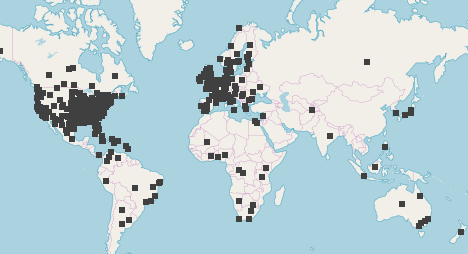
\includegraphics[scale=0.45]{resources/Geolokacija.png}
    \label{fig:Geolokacija}
    \caption{Geografksa rasprostranjenost autora uz osvrt na godine - gradijentni prelaz od plave (1950) do crvene (2010)}
\end{figure}

Lorem ipsum dolor sit amet, consectetur adipisicing elit, sed do eiusmod tempor incididunt ut labore et dolore magna aliqua. Ut enim ad minim veniam, quis nostrud exercitation ullamco laboris nisi ut aliquip ex ea commodo consequat. Duis aute irure dolor in reprehenderit in voluptate velit esse cillum dolore eu fugiat nulla pariatur. Excepteur sint occaecat cupidatat non proident, sunt in culpa qui officia deserunt mollit anim id est laborum.

Zastupljenost \v{z}anrova je prikazana na slici \ref{fig:ZastupljenostZanrova}.
\begin{figure}[H]
    \centering
    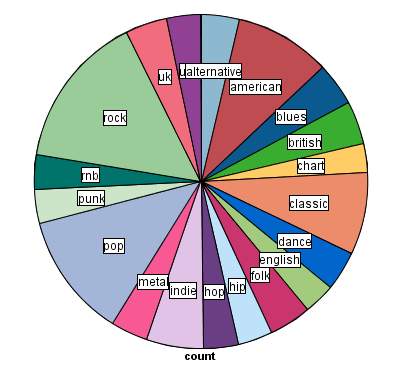
\includegraphics[scale=0.55]{resources/ZastupljenostZanrova.png}
    \label{fig:ZastupljenostZanrova}
    \caption{Zastupljenost \v{z}anrova}
\end{figure}

Lorem ipsum dolor sit amet, consectetur adipisicing elit, sed do eiusmod tempor incididunt ut labore et dolore magna aliqua. Ut enim ad minim veniam, quis nostrud exercitation ullamco laboris nisi ut aliquip ex ea commodo consequat. Duis aute irure dolor in reprehenderit in voluptate velit esse cillum dolore eu fugiat nulla pariatur. Excepteur sint occaecat cupidatat non proident, sunt in culpa qui officia deserunt mollit anim id est laborum.

Zavisnost du\v{z}ine pesama u odnosu na godinu nastanka prikazana je na slici \ref{fig:YearDuration}.
\begin{figure}[H]
    \centering
    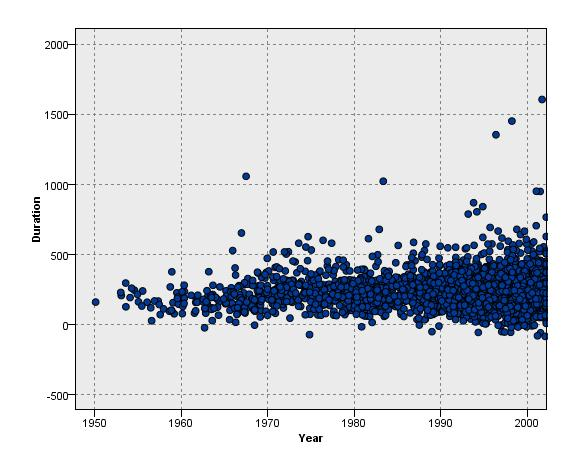
\includegraphics[scale=0.4]{resources/year-duration.jpg}
    \label{fig:YearDuration}
    \caption{Odnos godine i du\v{z}ine pesama}
\end{figure}

Lorem ipsum dolor sit amet, consectetur adipisicing elit, sed do eiusmod tempor incididunt ut labore et dolore magna aliqua. Ut enim ad minim veniam, quis nostrud exercitation ullamco laboris nisi ut aliquip ex ea commodo consequat. Duis aute irure dolor in reprehenderit in voluptate velit esse cillum dolore eu fugiat nulla pariatur. Excepteur sint occaecat cupidatat non proident, sunt in culpa qui officia deserunt mollit anim id est laborum.

Lorem ipsum dolor sit amet, consectetur adipisicing elit, sed do eiusmod tempor incididunt ut labore et dolore magna aliqua. Ut enim ad minim veniam, quis nostrud exercitation ullamco laboris nisi ut aliquip ex ea commodo consequat. Duis aute irure dolor in reprehenderit in voluptate velit esse cillum dolore eu fugiat nulla pariatur. Excepteur sint occaecat cupidatat non proident, sunt in culpa qui officia deserunt mollit anim id est laborum.

\section{Pravila pridruzivanja}
\label{sec:PravilaPridruzivanja}

Uo\v{c}avanje zavisnosti izmedju atributa je uradjeno kori\v{s}\'c{}enjem algoritma \emph{Apriori}. Najpre, kao \v{s}to je opisano u poglavlju \ref{sec:Preprocesiranje}, bilo je potrebno eleminisati slogove koji sadr\v{z}e nedostaju\'c{}e vrednosti na relevantnim atributima. Slede\'c{}i korak je zavisio od toga koje su zavisnosti analizirane. Poku\v{s}ali smo da pronadjemo zavisnosti izmedju zanrova, drzava i vremena kreiranja pesme. Rezultati rada Apriori algoritma slede u nastavku. Svi rezultati prikazani ispod su samo deo \v{c}itavog skupa rezultata, izabrani jer smo smatrali da su najinteresantnija.


\subsection{Zavisnosti izmedju \v{z}anrova}
\label{subsec:AprioriZavisnostZanrova}

Nakon prilagodjavanja atributa \emph{\v{z}anr} algoritmu, dobijeni su rezultati prikazani na slici \ref{fig:aprioriZanrovi}. Na njoj je prikazano 10 najizra\v{z}ajnijih pravila sortirana prvo po podr\v{s}ci, a zatim po lift meri, opadaju\'c{}e.
Ovi rezultati su relevantni iako su dobijeni na relativno malim skupom slogova.

\begin{figure}[H]
    \footnotesize
    \centering
    \begin{tabular}{|c|c|c|c|c|}
        \hline
        Podr\v{s}ka & Pouzdanost & Lift mera & Glava pravila & Telo pravila \\
        \hline
        0.2646 & 0.7404 & 1.5567 & rock & pop \\
        0.2646 & 0.5563 & 1.5567 & pop & rock \\
        0.2248 & 0.9930 & 2.0878 & rock & classic \\
        0.2163 & 0.8176 & 3.6114 & classic & pop, rock \\
        0.2163 & 0.9623 & 2.6926 & pop & rock, classic \\
        0.2163 & 1.0000 & 2.1026 & rock & pop, classic \\
        0.1612 & 0.9967 & 2.0957 & rock & indie \\
        0.1405 & 0.9170 & 5.9225 & british & uk \\
        0.1405 & 0.9075 & 5.9225 & uk & british \\
        0.1373 & 0.5582 & 1.1736 & rock & american, classic \\
        \hline
    \end{tabular}
    \caption{Rezultati Apriori algoritma koji pokazuju zavisnost medju \v{z}anrovima}
    \label{fig:aprioriZanrovi}
\end{figure}


\subsection{Zavisnost \v{z}anra od decenije}
\label{subsec:AprioriZavisnostZanraOdDecenije}

Istra\v{z}ivanje koji je \v{z}anr bio zastupljen u nekoj deceniji je dalo no\v{c}ekivane rezultate. Na tabeli \ref{fig:aprioriDecade} prikazana su dobijena pravila zavisnosti sortirana prvo po podr\v{s}ci, a zatim po lift meri, opadaju\'c{}e.
Kako se kasnije vidi na slici \ref{fig:YearDuration}, najve\'c{}i deo skupa obradjenih podataka pripada dvehiljaditim godinama. Zbog ovoga se dobijeni rezulati koncentri\v{s}u na ovoj deceniji. Kori\v{s}enje ve\'c{}eg i raznovrsnijeg skupa podataka bi doneo druga\v{c}ije rezultate.

\begin{figure}[H]
    \footnotesize
    \centering
    \begin{tabular}{|c|c|c|c|c|}
        \hline
        Podr\v{s}ka & Pouzdanost & Lift mera & Glava pravila & Telo pravila \\
        \hline
        0.0716 & 0.8133 & 1.6369 & 00s & pop, chart \\
        0.0525 & 0.7857 & 1.5815 & 00s & rnb, hop, hall, dance, hip \\
        0.0764 & 0.7385 & 1.4864 & 00s & dance \\
        0.0615 & 0.6824 & 1.3734 & 00s & rnb \\
        0.0615 & 0.6667 & 1.3419 & 00s & hop hip \\
        0.0541 & 0.6000 & 1.2077 & 00s & metal \\
        0.0530 & 0.5917 & 1.1910 & 00s & rock, alternative \\
        0.0578 & 0.5619 & 1.1309 & 00s & alternative \\
        0.0896 & 0.5541 & 1.1153 & 00s & indie \\
        0.0891 & 0.5526 & 1.1123 & 00s & rock, indie \\
        \hline
    \end{tabular}
    \caption{Rezultati Apriori algoritma koji pokazuju zavisnost izmedju \v{z}anrova i decenija tokom koje su bili popularni}
    \label{fig:aprioriDecade}
\end{figure}


\subsection{Zavisnost \v{z}anra od lokacije}
\label{subsec:AprioriZavisnostZanraOdLokacije}

Lokacija autora je atribut \v{c}ije ja vrednost \v{c}esto nepostoju\'c{}a. A ukoliko jeste, iste lokacije su na razli\v{c}itim pesmama druga\v{c}ije napisane. Na primer, jedna pesma ima lokaciju \emph{London}, a druga \emph{London, UK}. Ovakvi podaci su doveli do lo\v{s}ih rezultata istra\v{z}ivanja - slika \ref{fig:aprioriLocation}. Nazalost, jedina pravila koja imaju dovoljno veliku pouzdanost su oblika:
$$\{\emph{uk, british}\} \rightarrow \emph{England}$$
Ovo nam nije od preteranog zna\v{c}aja jer je o\v{c}ekivano da se u Engleskoj slu\v{s}aju pesme \v{z}anra \emph{british}.

\begin{figure}[H]
    \footnotesize
    \centering
    \begin{tabular}{|c|c|c|c|c|}
        \hline
        Podr\v{s}ka & Pouzdanost & Lift mera & Glava pravila & Telo pravila \\
        \hline
        0.0525 & 0.8684 & 7.6535 & England & pop, rock, classic, uk, english, british \\
        0.0541 & 0.7786 & 6.8621 & England & pop, rock, classic, uk, british \\
        0.0546 & 0.8729 & 7.6928 & England & pop, rock, classic, and, english \\
        0.0546 & 0.8729 & 7.6928 & England & rock, classic, uk, english, british \\
        0.0557 & 0.8268 & 7.2865 & England & pop, and, uk, english, british \\
        \hline
    \end{tabular}
    \caption{Rezultati Apriori algoritma koji pokazuju zavisnost izmedju \v{z}anrova i lokacije}
    \label{fig:aprioriLocation}
\end{figure}

\section{Klasifikacija}
\label{sec:Klasifikacija}

Jedan od glavnih problema u \v{c}itavom skupu je veliki broj nedostaju\c'{}ih vrednosti za zanr. Stoga smo poku\v{s}ali da napravimo klasifikator koji \'c{}e klasifikovati instance sa nepoznatim vrednostima za \v{z}anr, treniran nad onim podacima gde su te informacije dostupne.

Prvi problem na koji smo nai\v{s}li su nestandarne vrednosti za \v{z}anr (videti poglavlje \ref{sec:Preprocesiranje}), stoga smo kori\v{s}\'c{}enjem jednostavnih transformacija izvukli slogove sa nedvosmislenom vredno\v{s}\'c{}u za \v{z}anr, a eliminisali one koji su za \v{z}anr imali vrednosti koje nisu bile od zna\v{c}aja za analizu (neki slogovi su imali vi\v{s}e razli\v{c}tih \v{z}anrova). Takodje smo neke sli\v{c}ne \v{z}anrove spojili u jedan, zarad jednostavnijeg rada (na primer \emph{jazz} i \emph{blues} se \v{c}esto pojavljuju zajedno ih ima smisla posmatrati kao jedan \v{z}anr).

Za predikciju vrednosti \v{z}anra smo koristili atribite \emph{loudness}, \emph{tempo} i \emph{mode}. Na\v{z}alost, iz njihove prostorne rasprostranjenosti se vidi da ne postoji jednostavni separator instanci raznih klasa - slika \ref{fig:ZanrKlasifikacija}. Odlu\v{c}ili smo da isprobamo \emph{KNN} algoritam u nadi da \'c{}e male grupe pesama istog \v{z}anra lepo klasifikovati bliske instance. O\v{c}ekivano, najbolji model koji smo dobili je imao preciznost od $52.65\%$. Na slici \ref{fig:KNNgreske} se mo\v{z}e videti kako se gre\v{s}ka menjala sa razli\v{c}itim vrednostima za parametar $k$.

\begin{figure}[H]
    \centering
    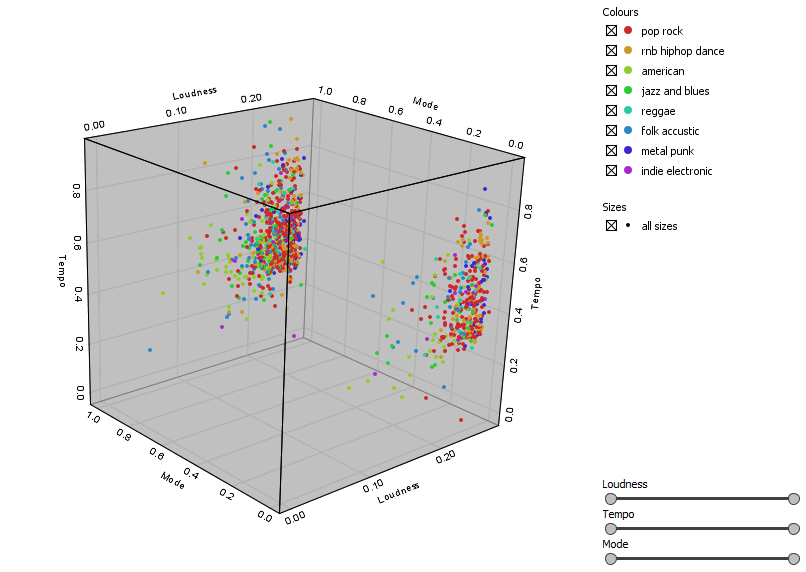
\includegraphics[scale=0.5]{resources/genre_scatter.PNG}
    \caption{3D prikaz pesama razli\v{c}itih \v{z}anrova u prostoru sa koordinatama \emph{loudness}, \emph{tempo} i \emph{mode}}
    \label{fig:ZanrKlasifikacija}
\end{figure}

\begin{figure}[H]
    \centering
    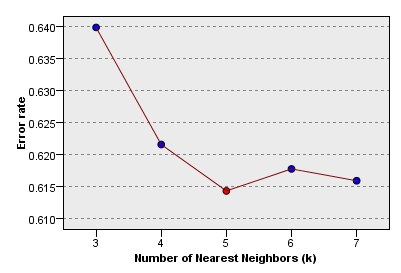
\includegraphics{resources/KNN_errors.PNG}
    \caption{Gre\v{s}ke dobijene za kreirane modele $k$ parametrom u opsegu $[3,7]$}
    \label{fig:KNNgreske}
\end{figure}

Ono \v{s}to nismo o\v{c}ekivali je jednaka va\v{z}nost atributa prilikom pravljenja klasifikatora - slika \ref{fig:KNNvaznost}. Intuicija nekako ka\v{z}e da su ja\v{c}e pesme podlo\v{z}nije da budu \v{z}anra \emph{metal}, ali rezultati su pobili tu intuiciju.

\begin{figure}[H]
    \centering
    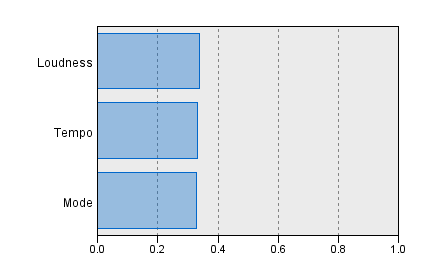
\includegraphics[scale=0.7]{resources/KNN_pred_imp.PNG}
    \caption{Va\v{z}nost atributa prilikom klasifikacije}
    \label{fig:KNNvaznost}
\end{figure}

\section{Klasterovanje}
\label{sec:Klasterovanje}

Isprobali smo razli\v{c}ite algoritme klasterovanja. Po\v{c}etna ideja je bila da na taj na\v{c}in izdvojimo grupe pesama koje su sli\v{c}ne i prema tome formiramo liste pesama. Ovu ideju smo sproveli algoritmima K-sredina, K-medioida, DBSCAN i algoritmom hijerarhijskog klasterovanja. Medjutim, dobijeni rezultati nisu bili zadovoljavaju\'c{}i te ne\'c{}emo ulaziti u njihovu dublju analizu.

Na slici \ref{fig:knime-klasterovanje} prikazan je KNIME workflow koji smo koristili za isprobavanje algoritama.

\begin{figure}[H]
    \centering
    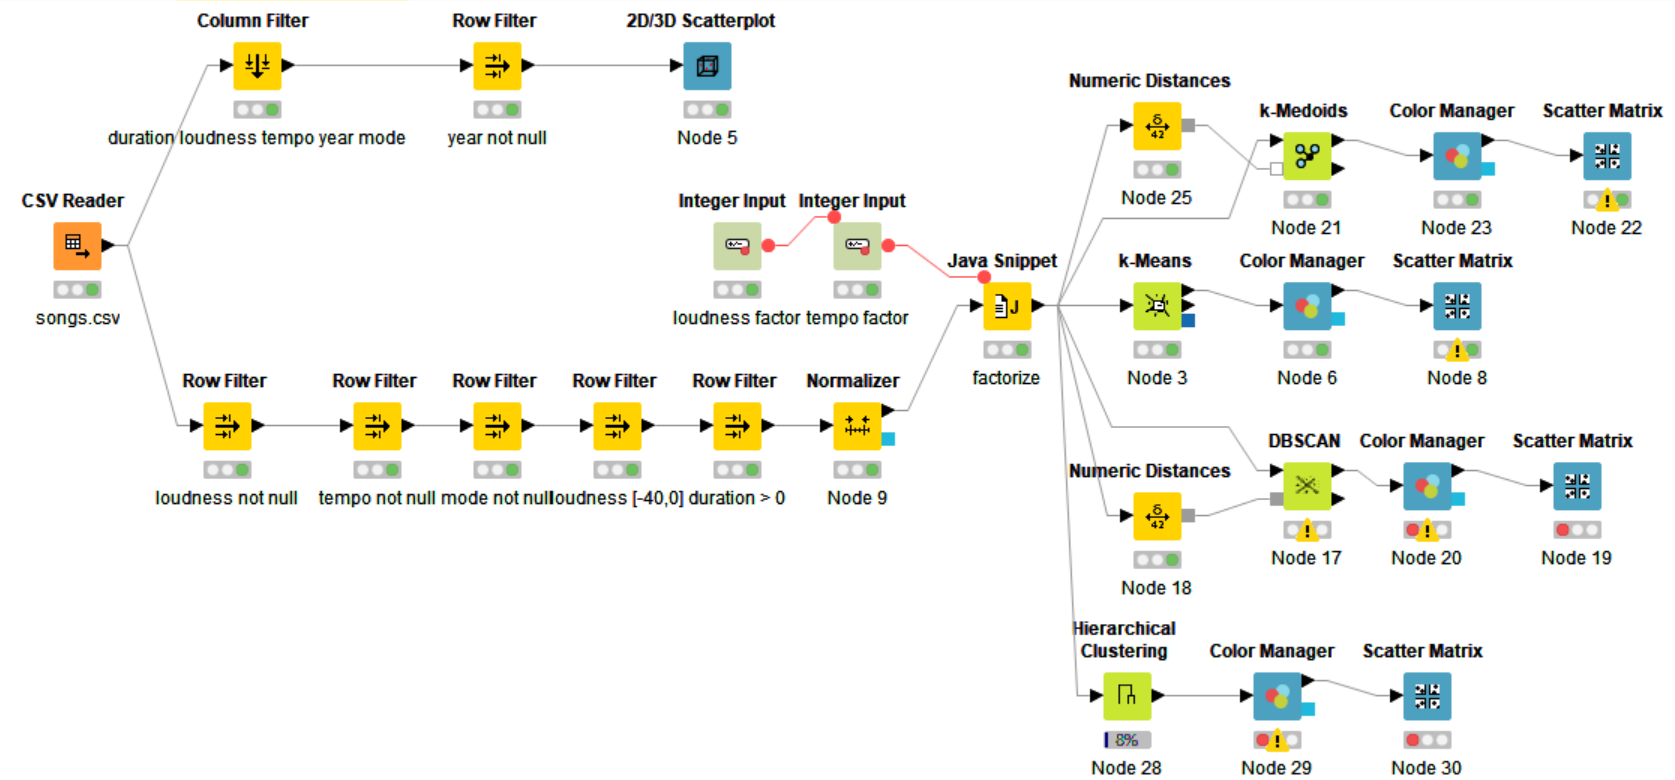
\includegraphics[scale=0.5]{KNIME-workflows/screenshots/klasterovanje.PNG}
    \caption{KNIME workflow za algoritme klasterovanja}
    \label{fig:knime-klasterovanje}
\end{figure}



\section{Zaključak}
\label{sec:Zakljucak}

Zakljucak... TODO

Lorem ipsum dolor sit amet, consectetur adipisicing elit, sed do eiusmod tempor incididunt ut labore et dolore magna aliqua. Ut enim ad minim veniam, quis nostrud exercitation ullamco laboris nisi ut aliquip ex ea commodo consequat. Duis aute irure dolor in reprehenderit in voluptate velit esse cillum dolore eu fugiat nulla pariatur. Excepteur sint occaecat cupidatat non proident, sunt in culpa qui officia deserunt mollit anim id est laborum.


\addcontentsline{toc}{section}{Literatura}
\bibliographystyle{plain}
\bibliography{literatura}

\newpage

\begin{appendices}
\section{Primer sloga}
\label{sec:DodatakPrimer}

\begin{figure}[H]
    \lstset{style=mystyle}
    \begin{lstlisting}[language=C, basicstyle=\footnotesize, numbers=none]
        analysis_sample_rate: 22050
        artist_7digitalid: 61424
        artist_familiarity: 0.5467275539627645
        artist_hotttnesss: 0.3861804160792181
        artist_id: ARE26EG1187B990AEF
        artist_latitude: 51.77045
        artist_location: Essex, England
        artist_longitude: 0.64255
        artist_mbid: de212b3a-2f54-4def-a13d-5a877bfaeaf7
        artist_mbtags: shape = (6,)
        artist_mbtags_count: shape = (6,)
        artist_name: Sunscreem
        artist_playmeid: 19156
        artist_terms: shape = (44,)
        artist_terms_freq: shape = (44,)
        artist_terms_weight: shape = (44,)
        audio_md5: c2f7f92e66d18e86af3752478d3be966
        bars_confidence: shape = (123,)
        bars_start: shape = (123,)
        beats_confidence: shape = (497,)
        beats_start: shape = (497,)
        danceability: 0.0
        duration: 232.4371
        end_of_fade_in: 0.0
        energy: 0.0
        key: 11
        key_confidence: 0.625
        loudness: -8.955
        mode: 0
        mode_confidence: 0.558
        release: Looking At You: The Club Anthems
        release_7digitalid: 196929
        sections_confidence: shape = (6,)
        sections_start: shape = (6,)
        segments_confidence: shape = (1045,)
        segments_loudness_max: shape = (1045,)
        segments_loudness_max_time: shape = (1045,)
        segments_loudness_start: shape = (1045,)
        segments_pitches: shape = (1045, 12)
        segments_start: shape = (1045,)
        segments_timbre: shape = (1045, 12)
        similar_artists: shape = (100,)
        song_hotttnesss: nan
        song_id: SOICLQB12A8C13637C
        start_of_fade_out: 232.437
        tatums_confidence: shape = (993,)
        tatums_start: shape = (993,)
        tempo: 130.201
        time_signature: 4
        time_signature_confidence: 0.0
        title: Exodus
        track_7digitalid: 2140010
        track_id: TRBBBLA128F424E963
        year: 1995
    \end{lstlisting}
    \caption{Primer sloga}
    \label{primer:Song}
\end{figure}

\section{Dodatak}
\label{sec:DodatakIzvlacenje}

\begin{figure}
\lstset{style=mystyle}
\begin{lstlisting}[language=Python, basicstyle=\footnotesize]
"""
Alexis Greenstreet (October 4, 2015) University of Wisconsin-Madison
"""
outputFile1 = open('SongCSV.csv', 'w')
csvRowString = ""

csvRowString = ("SongID,AlbumID,AlbumName,ArtistID,ArtistLatitude,ArtistLocation,"+
    "ArtistLongitude,ArtistName,Danceability,Duration,KeySignature,"+
    "KeySignatureConfidence,Loudness,Tempo,TimeSignature,TimeSignatureConfidence,"+
    "Title,Year,ArtistFamiliarity,ArtistHotttnesss,AudioMd5,EndOfFadeIn," + "Energy,Key,KeyConfidence,Mode,ModeConfidence,Release,SongHotttness,StartOfFadeOut,TrackId,Genre")
	csvAttributeList = re.split('\W+', csvRowString)
for i, v in enumerate(csvAttributeList):
    csvAttributeList[i] = csvAttributeList[i].lower()
outputFile1.write("SongNumber,");
outputFile1.write(csvRowString + "\n");
csvRowString = ""

#################################################
#Set the basedir here, the root directory from which the search
basedir = "/home/m/Documents/MillionSongSubset/data"
ext = ".h5"
#################################################

csvRowStringTotal = ""

for root, dirs, files in os.walk(basedir):
    files = glob.glob(os.path.join(root,'*'+ext))
    for f in files:
        print f

        songH5File = hdf5_getters.open_h5_file_read(f)
        song = Song(str(hdf5_getters.get_song_id(songH5File)))

        song.artistID = str(hdf5_getters.get_artist_id(songH5File))
        song.albumID = str(hdf5_getters.get_release_7digitalid(songH5File))
        song.albumName = str(hdf5_getters.get_release(songH5File))
        song.artistLatitude = str(hdf5_getters.get_artist_latitude(songH5File))
        if song.artistLatitude == 'nan':
            song.artistLatitude = ''
        song.artistLocation = str(hdf5_getters.get_artist_location(songH5File))
        song.artistLongitude = str(hdf5_getters.get_artist_longitude(songH5File))
        if song.artistLongitude == 'nan':
            song.artistLongitude = ''
        song.artistName = str(hdf5_getters.get_artist_name(songH5File))
        song.danceability = hdf5_getters.get_danceability(songH5File)
        if song.danceability == 0:
            song.danceability = ''
        else:
            song.danceability = str(song.danceability)
        song.duration = str(hdf5_getters.get_duration(songH5File))
        song.keySignature = str(hdf5_getters.get_key(songH5File))
        song.keySignatureConfidence = str(hdf5_getters.get_key_confidence(songH5File))
        song.loudness = str(hdf5_getters.get_loudness(songH5File))
        song.tempo = str(hdf5_getters.get_tempo(songH5File))
        song.timeSignature = str(hdf5_getters.get_time_signature(songH5File))
        song.timeSignatureConfidence = str(hdf5_getters.get_time_signature_confidence(songH5File))
        song.title = str(hdf5_getters.get_title(songH5File))
        song.year = str(hdf5_getters.get_year(songH5File))
        if song.year == '0':
            song.year = ''
        song.artistFamiliarity = str(hdf5_getters.get_artist_familiarity(songH5File))
        song.artistHotttnesss = str(hdf5_getters.get_artist_hotttnesss(songH5File))
        song.audioMd5 = str(hdf5_getters.get_audio_md5(songH5File))
        song.endOfFadeIn = str(hdf5_getters.get_end_of_fade_in(songH5File))
        song.energy = str(hdf5_getters.get_energy(songH5File))
        song.key = str(hdf5_getters.get_key(songH5File))
        song.keyConfidence = str(hdf5_getters.get_key_confidence(songH5File))
        song.mode = str(hdf5_getters.get_mode(songH5File))
        song.modeConfidence = str(hdf5_getters.get_mode_confidence(songH5File))
        song.release = str(hdf5_getters.get_release(songH5File))
        song.startOfFadeOut = str(hdf5_getters.get_start_of_fade_out(songH5File))
        song.songHotttness = str(hdf5_getters.get_song_hotttnesss(songH5File))
        if song.songHotttness == 'nan':
            song.songHotttness = ''
        song.trackId = str(hdf5_getters.get_track_id(songH5File))
        artistMbtags = np.array(hdf5_getters.get_artist_mbtags(songH5File))
        song.genre = ' | '.join(artistMbtags)

        csvRowString += str(song.songCount) + ","
        csvRowString += song.id + ","
        csvRowString += song.albumID + ","
        csvRowString += song.albumName.replace(',',"") + ","
        csvRowString += song.artistID + ","
        csvRowString += song.artistLatitude + ","
        csvRowString += song.artistLocation.replace(',','') + ","
        csvRowString += song.artistLongitude + ","
        csvRowString += song.artistName.replace('"',"") + ","
        csvRowString += song.danceability + ","
        csvRowString += song.duration + ","
        csvRowString += song.keySignature + ","
        csvRowString += song.keySignatureConfidence + ","
        csvRowString += song.loudness + ","
        csvRowString += song.tempo + ","
        csvRowString += song.timeSignature + ","
        csvRowString += song.timeSignatureConfidence + ","
        csvRowString += song.title.replace('"',"") + ","
        csvRowString += song.year + ","
        csvRowString += song.artistFamiliarity + ","
        csvRowString += song.artistHotttnesss + ","
        csvRowString += song.audioMd5 + ","
        csvRowString += song.endOfFadeIn + ","
        csvRowString += song.energy + ","
        csvRowString += song.key + ","
        csvRowString += song.keyConfidence + ","
        csvRowString += song.mode + ","
        csvRowString += song.modeConfidence + ","
        csvRowString += song.release + ","
        csvRowString += song.songHotttness + ","
        csvRowString += song.startOfFadeOut + ","
        csvRowString += song.trackId + ","
        csvRowString += song.genre + "\n"
        csvRowStringTotal += csvRowString
        csvRowString = ""

        songH5File.close()

outputFile1.write(csvRowStringTotal)
outputFile1.close()
\end{lstlisting}
\label{code:ConvertToCSV}
\caption{Skript kori\v{s}\'c{}en za konvertovanje iz HDF5 u CSV format.}
\end{figure}

\section{Statistika skupa podataka}
\label{sec:Statistika}

\begin{figure}[H]
\centering
\small
\Rotatebox{90}{%
    \begin{tabular}{|c|c|c|c|c|c|c|c|}
        \hline
        Column & ArtistLatitude & Duration & Loudness & Tempo & Year & Energy & Mode \\
        \hline
        Min & -41.281 & -114 & -51.643 & 0 & 1 & 0 & 0 \\
        Max & 151246 & 1815.222 & 261.538 & 262.828 & 2010 & 0.399 & 1 \\
        Mean & 94.001 & 238.379 & -10.444 & 122.868 & 1996.381 & 7.614E-05 & 0.691 \\
        Std. deviation & 2641.518 & 113.117 & 6.217 & 35.216 & 42.910 & 0.005 & 0.462 \\
        Variance & 6977616.187 & 12795.546 & 38.644 & 1240.182 & 1841.236 & 2.893E-05 & 0.21363 \\
        Skewness & 52.760 & 3.20372 & 8.711 & 0.404 & -43.0545 & 70.828 & -0.826 \\
        Kurtosis & 2922.508 & 24.813 & 396.106 & 0.487 & 1997.926 & 5029.175 & -1.319 \\
        Overall sum & 352221.307 & 2375926.299 & -104109.426 & 1224748.712 & 9317112 & 0.758 & 6876 \\
        No. missings & 6251 & 31 & 30 & 30 & 331 & 44 & 44 \\
        No. NaNs & 0 & 0 & 0 & 0 & 0 & 0 & 0 \\
        \hline
    \end{tabular}
}%
\caption{Statistike nama relevantnih atributa iz skupa}
\label{table:stats}
\end{figure}

\end{appendices}


\end{document}
